\chapter{Introduction}

	\section{Relative Camera Pose}
		Equations to transform pose in world coordinates to relative pose with respect to the coordinate frame of the first camera.

	\section{Rotation Metrics}
	\cite{huynh2009metrics}
	
	\section{Two-Frame Structure from Motion}
	
	\section{Multiview Structure from Motion}
	
	\section{Camera Pose and Transformations}
		The camera pose, also known as the \emph{extrinsic parameters}, is a combination of position and orientation.
		Together, they define a coordinate transformation from the camera coordinate frame to the world coordinate frame.
		Such a transformation is commonly represented by a translation vector $\vectr{t} \in \R^3$ and a rotation matrix $\matr{R} \in SO(3)$. 
		Together, they describe a rigid transformation which can also be written as a $4 \times 4$ matrix of the form
		\begin{equation}
			\matr{T} = 
			\begin{bmatrix}
				\matr{R} 	& \vectr{t} \\
				0 			& 1
			\end{bmatrix} 
			\in SE(3).
		\end{equation}
		\todo{Insert a figure showing: world coordinate frame, camera coordinate frame, transformation matrix}
		
		In Structure from Motion, there is not only one camera, but many cameras with different transformations.
		This is also the case in this work, but the sequence of transformations is ordered according to the path of the camera motion. 
		Specifically, we deal with a sequence of rotations $\matr{R}_1, \dots, \matr{R}_n$ and translations $\vectr{t}_1, \dots, \vectr{t}_n$. 
		Depending on how the poses are obtained, they are all relative to a common (world) coordinate frame.
		Sometimes it is useful to have the coordinate frame of the first camera transform be the common frame for all transformations.
		This can be achieved by applying the transformations
		\begin{align}\label{eq:relative_rotation_conversion}
			\begin{split}
				\matr{R}_{i}^\prime 	&= \matr{R}_{1}^{\top} \matr{R}_{i} \\
				\vectr{t}_{i}^\prime 	&= \matr{R}_{1}^{\top} (\vectr{t}_i - \vectr{t}_1)
			\end{split}
		\end{align}
%		\begin{equation}
%			\matr{R}_{i \rightarrow 1} 	= \matr{R}_{\text{w} \rightarrow 1} \matr{R}_{i \rightarrow \text{w}}
%										= \matr{R}_{1 \rightarrow \text{w}}^{-1} \matr{R}_{i \rightarrow \text{w}}
%										= \matr{R}_{1 \rightarrow \text{w}}^{\top} \matr{R}_{i \rightarrow \text{w}}
%		\end{equation}
%		\begin{equation}
%		\vectr{t}_{i \rightarrow 1} = \matr{R}_{1 \rightarrow \text{w}}^{\top} (\vectr{t}_i - \vectr{t}_1)
%		\end{equation}
		to get the new relative rotation $\matr{R}_{i}^\prime$ and relative translation $\vectr{t}_{i}^\prime$.
		Note that for $i = 1$ we obtain $\matr{R}_{1}^\prime = \matr{I}$ and $\vectr{t}_{1}^\prime = \vectr{0}$.
		
		\noindent\rule{2cm}{0.4pt}
		\todo{make good transition}
		
		So far, we have seen rotations represented as matrices. 
		However, it is redundant to describe rotations with nine numbers when in fact there are only three degrees of freedom for a three-dimensional rotation, i.e. two degrees for the orientation of the axis and one for the angle of rotation around the axis.
		It is also not straightforward to interpolate rotations in $SO(3)$, or to find the best approximation for a matrix that lies outside of $SO(3)$.\todo{citation needed}
		
		Below we discuss and compare three other popular representations used to describe rotations.
		A brief overview is also shown in table~\ref{tbl:comparison_representations_of_rotations}.
		\begin{table}
			\small
			\begin{center}
				\begin{tabular}{|l|p{2.5cm}|p{2.5cm}|p{2.5cm}|p{2.5cm}|}
					\hline
					& Euler angles & Matrix & Axis-angle & Unit quaternion \\ \hline
					Typical use case & Robotics, Avionics & Computer Graphics, Physics & Intermediate representation & Computer Graphics, Physics \\ \hline
					Constraint & None & Orthonormality & Unit norm axis & 4D unit sphere \\ \hline
					Disadvantage & Gimbal lock & Numerically unstable & & Less intuitive \\ \hline
					Interpolation & hard & hard & hard & easy \\ \hline
					Identity rotation & ambiguous & unique & ambiguous &unique \\ 
					\hline
				\end{tabular}
			\end{center}
			\caption[A comparison of representations for rotations]
					{A comparison of representations for rotations.}
			\label{tbl:comparison_representations_of_rotations}
		\end{table}
		
		\paragraph{Euler Angles}
%		The fact that rotations in 3D have three degrees of freedom means there are only three coordinates needed to identify a rotation. 
%		Euler angles are one such choice of coordinates.
		The Euler angles represent a rotation with three numbers 
		$\alpha, \beta, \gamma \in \left[0, 2\pi\right)$.
		There are many different conventions and definitions of these three angles and how they are applied.
		In this thesis, we apply the rotations in the following order. 
		The initial coordinate frame shall be denoted by $(x, y, z)$.
		\begin{enumerate}
			\item The coordinate frame is rotated around the $x$-axis with angle $\alpha$. 
			This results in a new coordinate frame $(x^\prime, y^\prime, z^\prime)$.
			\item Next, the system is rotated around the $y^\prime$-axis by angle $\beta$. 
			The new coordinate frame is $(x^{\prime\prime}, y^{\prime\prime}, z^{\prime\prime})$.
			\item Finally, we perform a rotation around axis $z^{\prime\prime}$ by angle $\gamma$ to obtain the desired orientation.
		\end{enumerate}
		Altogether these steps can be formalized by a multiplication of three matrices that define the rotations around the different axes. 
		The result is a rotation matrix
		\begin{equation}
			\matr{R}(\alpha, \beta, \gamma) =
			\matr{R}_{z^{\prime\prime}}^\gamma
			\matr{R}_{y^\prime}^\beta
			\matr{R}_{x}^\alpha
		\end{equation}
		defined by the Euler angles. 
		It can be shown that this representation covers all 3D rotations. \todo{citation needed}
		However, the Euler angle representation also comes with drawbacks.
%		For example, a linear interpolation in the Euler domain between two points $(\alpha_1, \beta_1, \gamma_1)$ and $(\alpha_2, \beta_2, \gamma_2)$ by varying a parameter $\lambda \in [0, 1]$ gives 
%		\begin{equation}
%			(\alpha, \beta, \gamma) = (1 - \lambda) (\alpha_1, \beta_1, \gamma_1) + \lambda (\alpha_2, \beta_2, \gamma_2).
%		\end{equation}
%		The rotations associated with the angles $(\alpha, \beta, \gamma)$ is not an optimal choice for an 
		
		
		\paragraph{Axis-Angle}\todo{TODO}
		
		\paragraph{Quaternions}
		Quaternions are four-dimensional numbers.
		They are an extension of the complex numbers\footnote{A more appropriate name is \emph{compound numbers}.\todo{disputable}}.
		Formally, a quaternion is defined as $\vectr{q} = w + \vectr{i}x + \vectr{j}y + \vectr{k}z$ where $w, x, y, z \in \R$ and $\vectr{i},\vectr{j}$ and $\vectr{k}$ are the basis elements of the quaternion space.
		The quaternion can also be written as a tuple $\vectr{q} = (w, x, y, z) \in \R^4$ by using the notation
		\begin{equation}
			\vectr{1} = 
			\begin{bmatrix}
				1 \\ 
				0 \\ 
				0 \\ 
				0
			\end{bmatrix},\quad
			\vectr{i} = 
			\begin{bmatrix}
				0 \\ 
				1 \\ 
				0 \\ 
				0
			\end{bmatrix},\quad
			\vectr{j} = 
			\begin{bmatrix}
				0 \\ 
				0 \\ 
				1 \\ 
				0
			\end{bmatrix},\quad
			\vectr{k} =
			\begin{bmatrix}
				0 \\ 
				0 \\ 
				0 \\ 
				1
			\end{bmatrix}.
		\end{equation}
		But quaternions are not just tuples of numbers. 
		They are equipped with a separate addition and multiplication.
		Addition is simply carried out element-wise as for vectors, whereas multiplication makes use of the distributive rule and the property
		\begin{equation}
			\vectr{i}^2 = \vectr{j}^2 = \vectr{k}^2 = \vectr{i}\vectr{j}\vectr{k} = -1.
		\end{equation}
		Furthermore, the norm of a quaternion is defined as
		\begin{equation}
			\lVert \vectr{q} \rVert = \sqrt{w^2 + x^2 + y^2 + z^2}.
		\end{equation}
		
		In this thesis, we are particularly interested in the subset of quaternions called the \emph{unit quaternions}. These are all the quaternions with unit norm, i.e. $\lVert \vectr{q} \rVert = 1$. 
		The quaternions of this form describe 3D rotations and can be parameterized by
		\begin{equation}
			\vectr{q} = 
			\cos\left(\tfrac{\theta}{2}\right) + 
			\sin\left(\tfrac{\theta}{2}\right) \left(a_1 \vectr{i} + a_2 \vectr{j} + a_3 \vectr{k}\right),
		\end{equation}
		where $\theta \in \R$ is the angle of rotation around a unit-length axis $\vectr{a} = (a_1, a_2, a_3) \in \R^3$.
		\todo{explain that quaternions are not unique representation of rotations, and that negative axis-angle is represented by the same quaternion}
	
	\section{Deep Feedforward Neural Networks}
	\todo{This summary is based on the deep learning book}
	\todo{show a figure for a feed forward network}
	A \emph{feedforward neural network} is a function mapping an input $\vectr{x}$ to an output $\vectr{y} = f(\vectr{x})$.
	For example, $\vectr{y} \in \{\text{dog}, \text{cat} \}$ could be the output of the function deciding whether an image $\vectr{x}$ contains a dog or a cat. 
	The reason it is called a \emph{deep network} is because $f$ is often a long chain of function compositions, e.g. 
	$f = f^{(n)} \circ  \ldots  \circ f^{(2)} \circ f^{(1)}$.
	The functions $f^{(1)}, \dots, f^{(n)}$ are called \emph{layers} and $n$ is the \emph{depth} of the network.
	Each layer performs a computation on the output of the previous layer, hence the name \emph{feedforward}.
	
	A feed forward network is best visualized as a graph\footnote{More precisely it is a DAG (directed acyclic graph). It does not allow loops.}, the so-called \emph{computational graph}.
	A node in the graph represents a single layer and the edges represent the flow of data (input/output).
	\todo{Should explain comp. graph in terms of neurons?}
	These networks build the foundation of deep learning.
	Why?
	Because in general $f$ is unknown and must be learned to solve a specific task.
	The practical approach to finding a suitable $f$ is to consider a family of functions $f_{\vectr{w}}$ defined by the \emph{parameters} $\vectr{w}$, also called \emph{weights}.
	For example, the layer $i$ in the network might be a linear function $f_{}^{(i)}(\vectr{x}) = \matr{W} \vectr{x}$ where the parameters of this layer are the elements of the matrix $\matr{W}$.
	
	The collective of all functions in the family is called the \emph{model}.
	To solve the task (e.g. classifying dogs and cats), one has to \emph{train} the model.
	In other words, one has to search through the space of all parameters $\vectr{w}$ to find the ones that perform the best.
	The performance is measured with the \emph{loss function} 
	$L(f_{\vectr{w}}(\vectr{x}), \vectr{y}) \in \R$ that compares the prediction 
	$\vectr{\hat{y}} = f_{\vectr{w}}(\vectr{x})$ with the \emph{ground truth} $\vectr{y}$ and gives a score how close they are.
	The ground truth comes from the dataset, which is the most important resource of knowledge for training a model.
	The dataset contains many samples $\vectr{x}^{(1)}, \dots, \vectr{x}^{(N)}$ each with a ground truth label 
	$\vectr{y}^{(1)}, \dots, \vectr{y}^{(N)}$, e.g. each dog image in the dataset has a label 'dog' and each image with a cat has the label 'cat'.
	
	The loss function is not only used to evaluate the performance of the model, but to find optimal parameters for the model as part of the training.
	In general, the objective is to minimize the loss function on the data, that is
	\begin{equation}\label{eq:optimal_parameter_neural_network}
		\vectr{w}^\ast = \argmin_{\vectr{w}} 
		\sum_{i = 1}^{N} 
			L(f_{\vectr{w}}(\vectr{x}^{(i)}), \vectr{y}^{(i)}).
	\end{equation}
	The resulting function $f_{\vectr{w}^\ast}$ is a solution that best satisfies the loss function on all the data.
	How can $\vectr{w}^\ast$ be found?
	A common way to minimize the loss is to use gradient descent.
	It is one of the most general purpose optimization algorithms.
	Gradient descent can find a local minimum of a function $F$ by iteratively stepping in the opposite direction of the gradient, which can be described by the update rule
	\begin{equation}
		\vectr{w} \leftarrow 
		\vectr{w} - \lambda \frac{\partial F(\vectr{w})}{\partial \vectr{w}}.
	\end{equation}
	The parameter $\vectr{w}$ converges close to a local minimum when a suitable learning rate $\lambda$ is chosen. \todo{citation needed / is "converge" the right word to use here?}
	
	%In the context of this experiment, $\vectr{w}$ are the model parameters and $F$ is the loss over the training data. 
	
	
	% Gradient computation with backpropagation
	% Gradient descent
	% 
	
	\section{Recurrent Neural Networks}
		\newcommand{\imagecourtesycolah}{Image courtesy Christopher Olah \mbox{\href{http://colah.github.io/}{(colah.github.io)}}}
		\todo{Need references to early works on RNNs}
		So far, we have looked at the feedforward network, which is function that maps an input $\vectr{x}$ to an output $\vectr{y} = f(\vectr{x})$.
		It will always compute the same output for the same input, independently of the input-output pairs it has seen before.
		Now consider a sequence $\vectr{x}_1, \dots, \vectr{x}_T$ of inputs (e.g. a sentence).
		How can we learn to predict an attribute that depends on the whole sequence (e.g. the sentiment of the sentence)?
		One way is to concatenate the sequence to one vector and use the feed-forward network.
		However, this will limit the sequence length to a fixed size and potentially requires more training data.
		\todo{need reference for this statement}.
		How do we model predictions for a variable sequence length?
		And what if we want also the output to be a sequence? 
		What if the output sequence needs to have a different length than the input sequence, such as in machine translation? 
		\todo{citation needed}
		
		This is where the recurrent neural network (RNN) comes into play.
		It is a function that maps each vector $\vectr{x}_t \in \R^n$ from the sequence to a hidden state
		\begin{eqnarray}
			\vectr{h}_t = R(\vectr{x}_t, \vectr{h}_{t-1}), & &t = 1, \dots, T
		\end{eqnarray}
		with the hidden state $\vectr{h}_{t-1} \in \R^d$ carried over from the previous prediction as a second input, where $d$ is called the \emph{hidden size} of the RNN. 
		The hidden state represents the accumulated knowledge from all previous inputs.
		This way, the output at each time step $t$ depends on the inputs from $\vectr{x}_1$ to $\vectr{x}_{t - 1}$.
		\begin{figure}[tb]
			\centering
			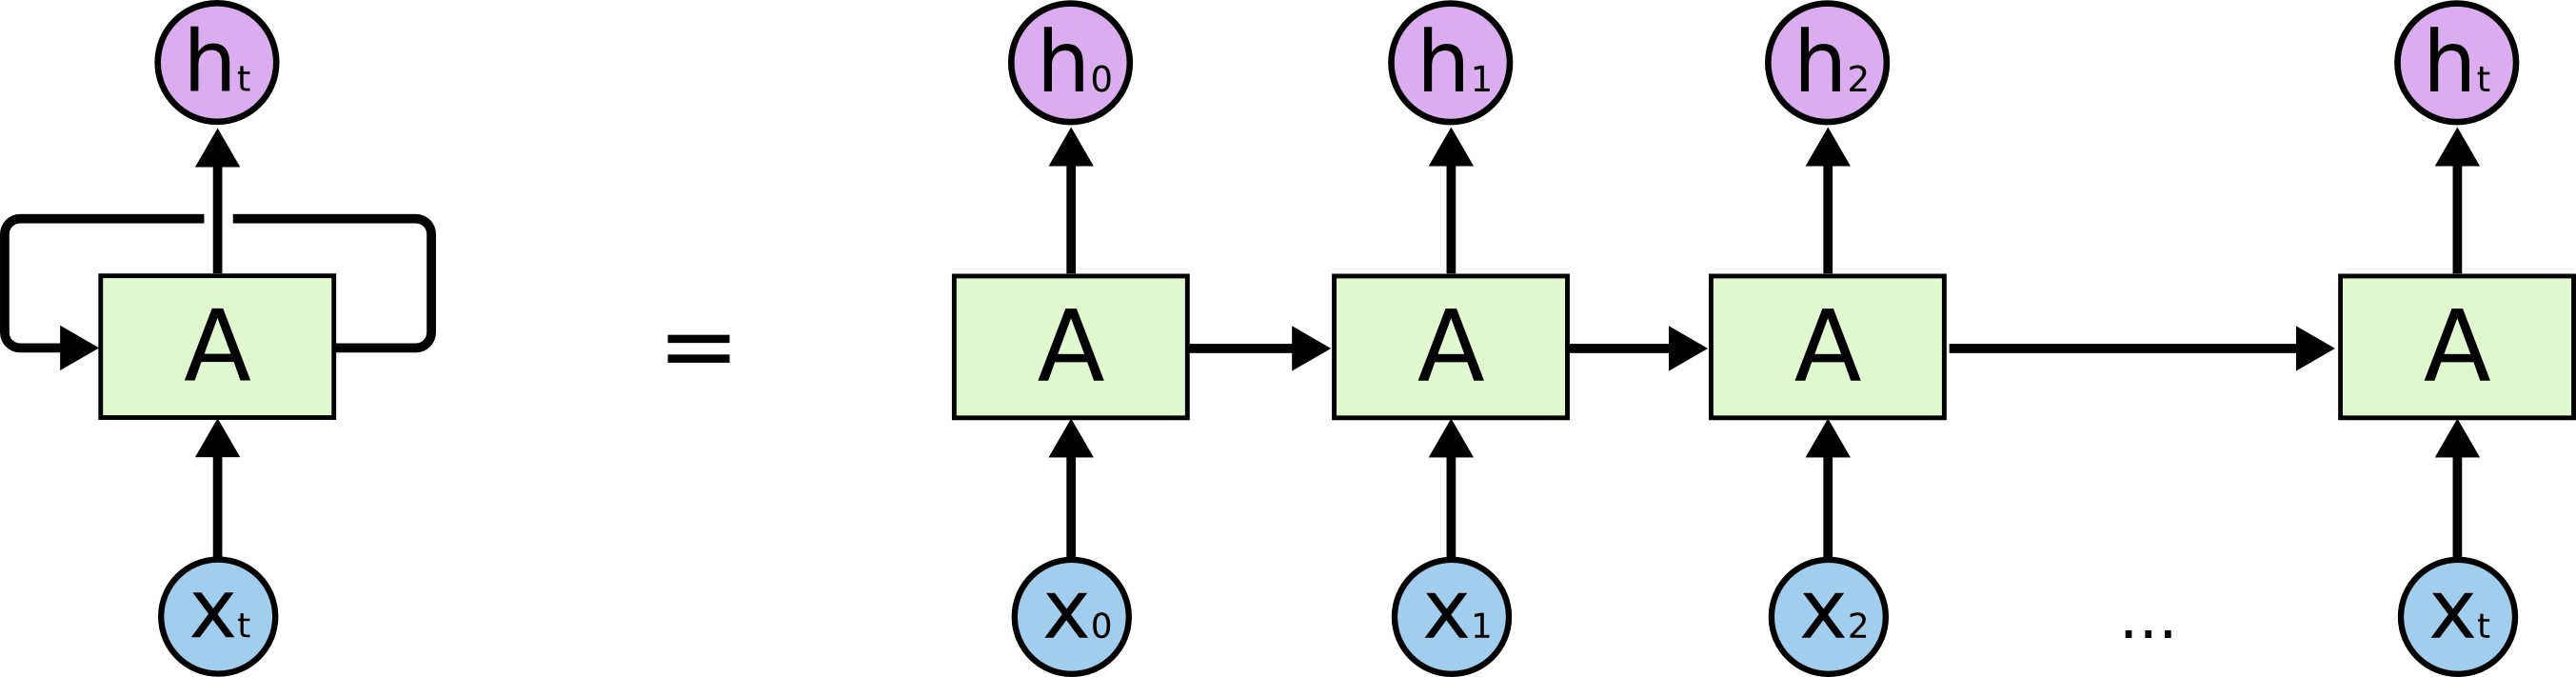
\includegraphics[width=0.9\linewidth]{Images/LSTM/RNN-unrolled}
			\caption[Unfolding the RNN]
			{Unfolding the RNN. Left: The RNN as a cyclic graph. 
				Right: Unfolded RNN for a number of timesteps.
				\imagecourtesycolah}
			\label{fig:RNN-unrolled}
		\end{figure}
		Figure~\ref{fig:RNN-unrolled} shows the RNN as a looping component.
		When unfolded, one can see the information flow from one state to the next.
		Note that it is possible to feed arbitrary sizes of sequences to the RNN.
		
		The simplest implementation of an RNN uses an affine transformation followed by a non-linear function:
		\begin{equation}
			\vectr{h}_t = 
			\tanh \left(
			\matr{W}
			\begin{bmatrix}
				\vectr{x}_t \\
				\vectr{h}_{t-1}
			\end{bmatrix}
			+ \vectr{b}
			\right)
		\end{equation}
		The weight matrix $\matr{W}$ has dimensions $d \times (n + d)$.
		Sometimes it is desirable to have an output that has a different size than the hidden state (e.g. for classification).
		In this case one can apply a second affine layer
		\begin{equation}
			\vectr{y}_t = \matr{V} \vectr{h}_t + \vectr{c}
		\end{equation}
		to obtain the prediction $\vectr{y}_t$.
		Otherwise we define the output as $\vectr{y}_t = \vectr{h}_t$.
		
		Training an RNN is not much different from a feed-forward network.
		The weights $\vectr{W}, \vectr{V}, \vectr{b}$ and $\vectr{c}$ are updated in the same fashion as for feed-forward networks using gradient descent on the loss function.
		Say we define a criterion $L_t(\vectr{y}_t, \vectr{\hat{y}}_t)$ for the loss between prediction and ground-truth at each time step $t$.
		Then, the total loss for the sequence is simply 
		\begin{equation}\label{eq:loss_for_rnn}
			L(\{\vectr{y}_1, \dots \vectr{y}_T\}, \{\vectr{\hat{y}}_1, \dots \vectr{\hat{y}}_T\}) = \sum_{t=1}^{T} L_t(\vectr{y}_t, \vectr{\hat{y}}_t).
		\end{equation}
		This loss will be used to compute gradients for updating the model parameters similar to feed-forward networks.
		
	\section{Gradient Computation for RNNs}
		
		The gradient computation is almost the same as for feed-forward networks and the back-propagation algorithm can be applied by unfolding the RNN as shown in figure~\ref{fig:RNN-unrolled}.
		However, there is a problem with the gradient computation in the above version of the RNN (\cite{pascanu2013difficulty}, \cite{bengio1994learning}).
		For long sequences, the gradient norm can become very small and this hurts the training.
		The RNN is not able to learn long-term dependencies when the gradient vanishes.
		To see this, let's write down the full equation for the gradient:
		\begin{equation}
			\frac{\partial L}{\partial \vectr{w}}
			= \sum_{t=1}^{T} 
				\frac{\partial L_t}{\partial \vectr{w}}
			= \sum_{t=1}^{T} 
				\sum_{k=0}^{t} 
					\frac{\partial L_t}{\partial \vectr{y}_t}
					\frac{\partial \vectr{y}_t}{\partial \vectr{h}_t}
					\left(
						\prod_{j=k+1}^{t} \frac{\partial \vectr{h}_j}{\partial \vectr{h}_{j-1}}
					\right)
					\frac{\partial \vectr{h}_{k}}{\partial \vectr{w}}
		\end{equation}
		In the above equation, we have the product term that causes the problem when the sequence is very long.
		Note that the partial derivatives are Jacobian matrices when we take the derivatives of a vector-valued function with respect to a vector.
		Due to many multiplications, the gradient values drop exponentially.
		\todo{Need a better explanation why values are <1 and drop exponentially}
		A more complete analysis is provided in \cite{pascanu2013difficulty}.
		
	\section{The Long Short-Term Memory}
		\begin{figure}[tb]
			\centering
			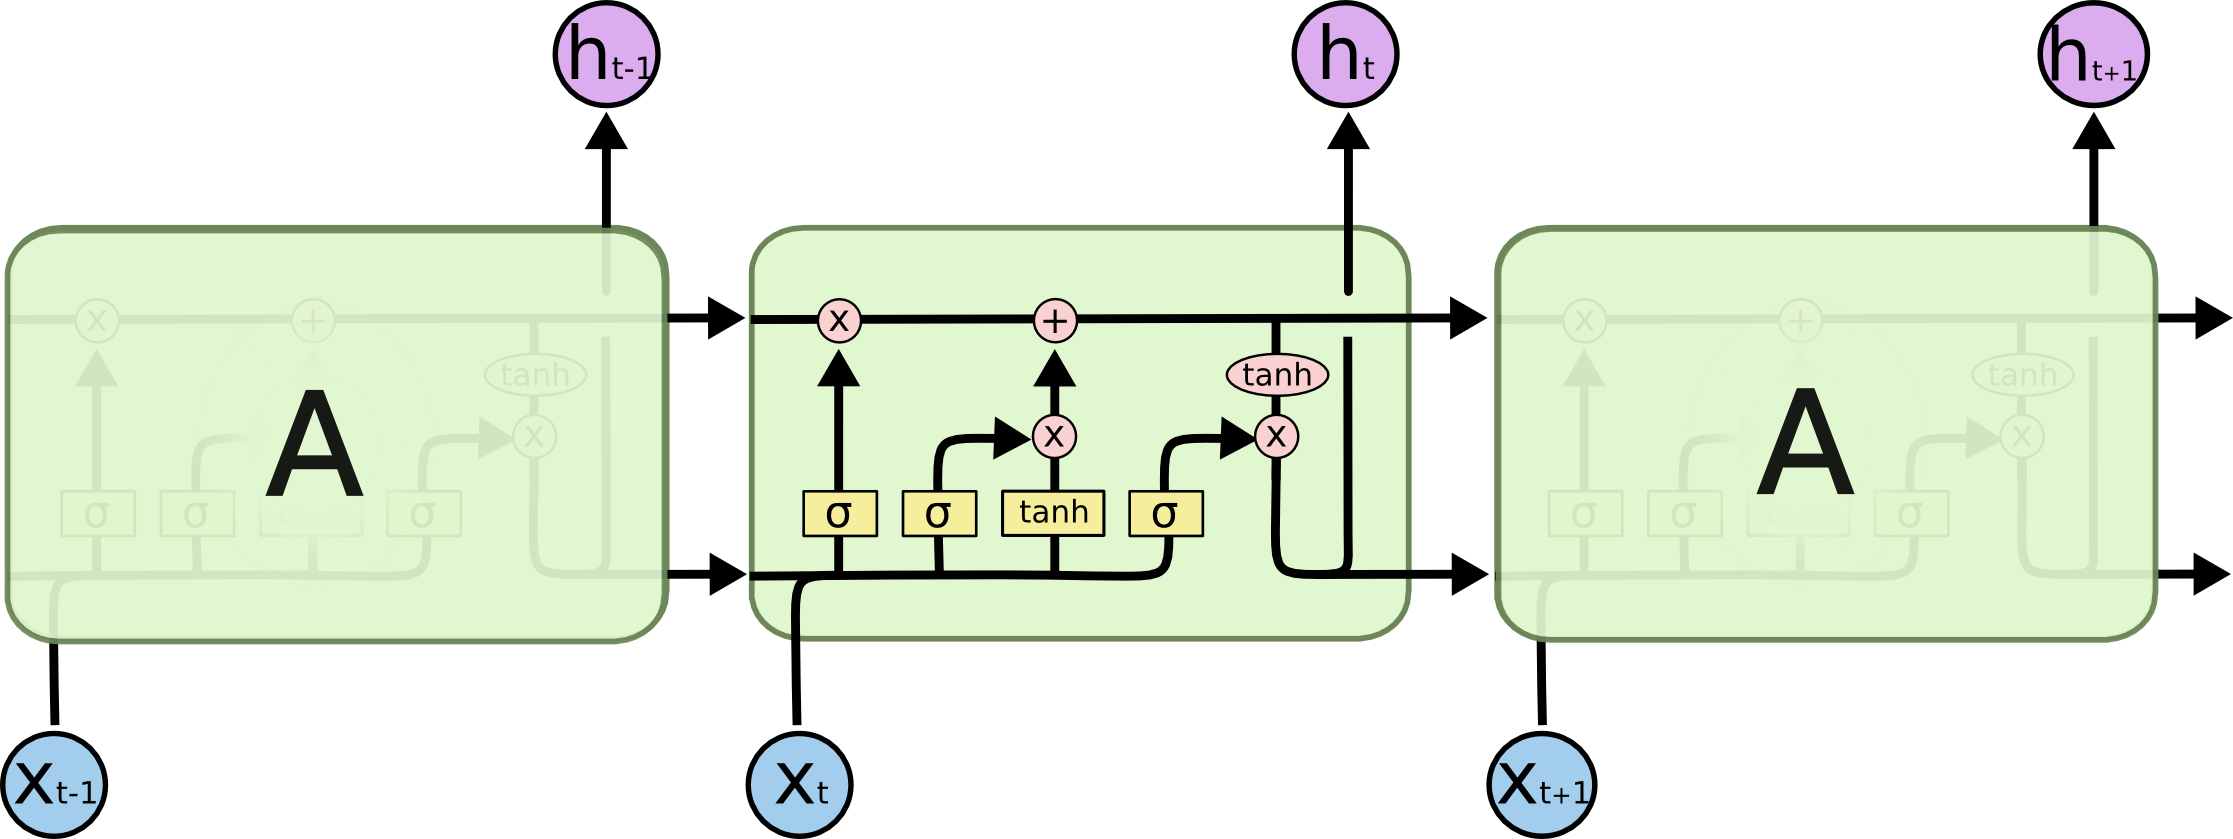
\includegraphics[width=0.9\linewidth]{Images/LSTM/LSTM3-chain}\\
			\vspace{5mm}
			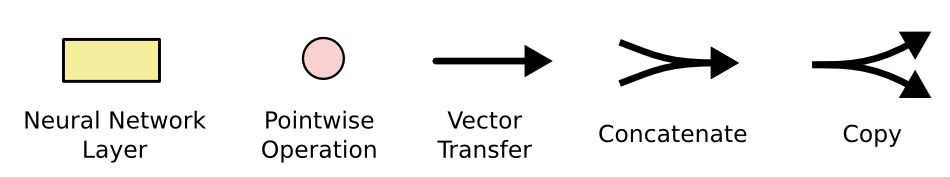
\includegraphics[width=0.5\linewidth]{Images/LSTM/LSTM2-notation}
			\caption[Unfolded LSTM cell]
					{Unfolded LSTM cell. 
					\imagecourtesycolah}
			\label{fig:LSTM3-chain}
		\end{figure}
		The Long Short-Term Memory (LSTM) is a version of the RNN that was designed to overcome the vanishing gradient problem described above, and it is also used in this thesis.
		As shown in figure~\ref{fig:LSTM3-chain}, it introduces four gates (in yellow) and an additional cell state variable that is carried over from one time step to the next.
		The recurrence can be formulated as a function 
		% $R \colon \R^n \times \R^d \times \R^d \rightarrow \R^d \times \R^d$
		\begin{align}\label{eq:LSTM_recurrence}
			(\vectr{h}_t, \vectr{c}_t) = R(\vectr{x}_t, \vectr{h}_{t-1}, \vectr{c}_{t-1}), & & t = 1, \dots, T.
		\end{align}
		More precisely, the hidden state and cell state are computed as follows:
		\begin{align}\label{eq:Vanilla-LSTM-Definition}
			\begin{split}
				\begin{bmatrix}
					\vectr{i} \\ 
					\vectr{f} \\ 
					\vectr{o} \\ 
					\vectr{g}
				\end{bmatrix}
				&=
				\begin{bmatrix}
					\sigma \\ 
					\sigma \\ 
					\sigma \\ 
					\tanh
				\end{bmatrix}
				\left(
				\matr{W}
				\begin{bmatrix}
					\vectr{x}_t \\
					\vectr{h}_{t-1}
				\end{bmatrix}
				+
				\begin{bmatrix}
					\vectr{b}_i \\ 
					\vectr{b}_f \\ 
					\vectr{b}_o \\ 
					\vectr{b}_g
				\end{bmatrix}
				\right)
				\\
				\vectr{c}_t &= \vectr{i} \odot \vectr{g} + \vectr{f} \odot \vectr{c}_{t-1} \\
				\vectr{h}_t &= \vectr{o} \odot \tanh(\vectr{c}_{t})
			\end{split}
		\end{align}
		The matrix $\matr{W} \in \R^{4d \times (n + d)}$ contains the weights for the input- and hidden state transformations before each gate.
		It can be broken down into four parts:
		\begin{align}
			\matr{W} &=
			\begin{bmatrix}
				\vectr{W}_i \\ 
				\vectr{W}_f \\ 
				\vectr{W}_o \\ 
				\vectr{W}_g
			\end{bmatrix}
		\end{align}
		We can see that there are three additional gates that control information flow with a sigmoid activation.
		If the sigmoid output is one, all information is let through, otherwise no information passes the gate. 
		
		The first is the input gate $\vectr{i}$.
		It controls how much information should be collected from the current input and hidden state.
		The second is the forget gate $\vectr{f}$, which will learn what information should be discarded from the previous cell state.
		Finally, the output gate $\vectr{o}$ regulates the amount of information that goes to the output $\vectr{h}_t$.
		
	\section{Training RNNs}
		There are several ways an RNN can be trained.
		
		% Many to many
		% Many to one
		% One to one
		% One to many
		
		% Using end of sequence token
		% How the hidden state is used between sequences
		%	Carry hidden state over
		%	Reset hidden state
		% 
		% How the ground truth is used
		% 	Does ground truth have same dimensionality as input?, as hidden state?
		%	
		
	\section{PyTorch}
		PyTorch is a deep learning framework for Python that comes with a rich tensor library.
		It differs from other libraries (TensorFlow, Caffe, Theano and more) in the sense that it builds the computational graph dynamically at runtime.
		This flexibility allows for controlling the computational flow while training or testing the network.